\subsection{The LTCC Window}


\paragraph{Re-fabricate windows}

\begin{figure}[h]
	\centering
	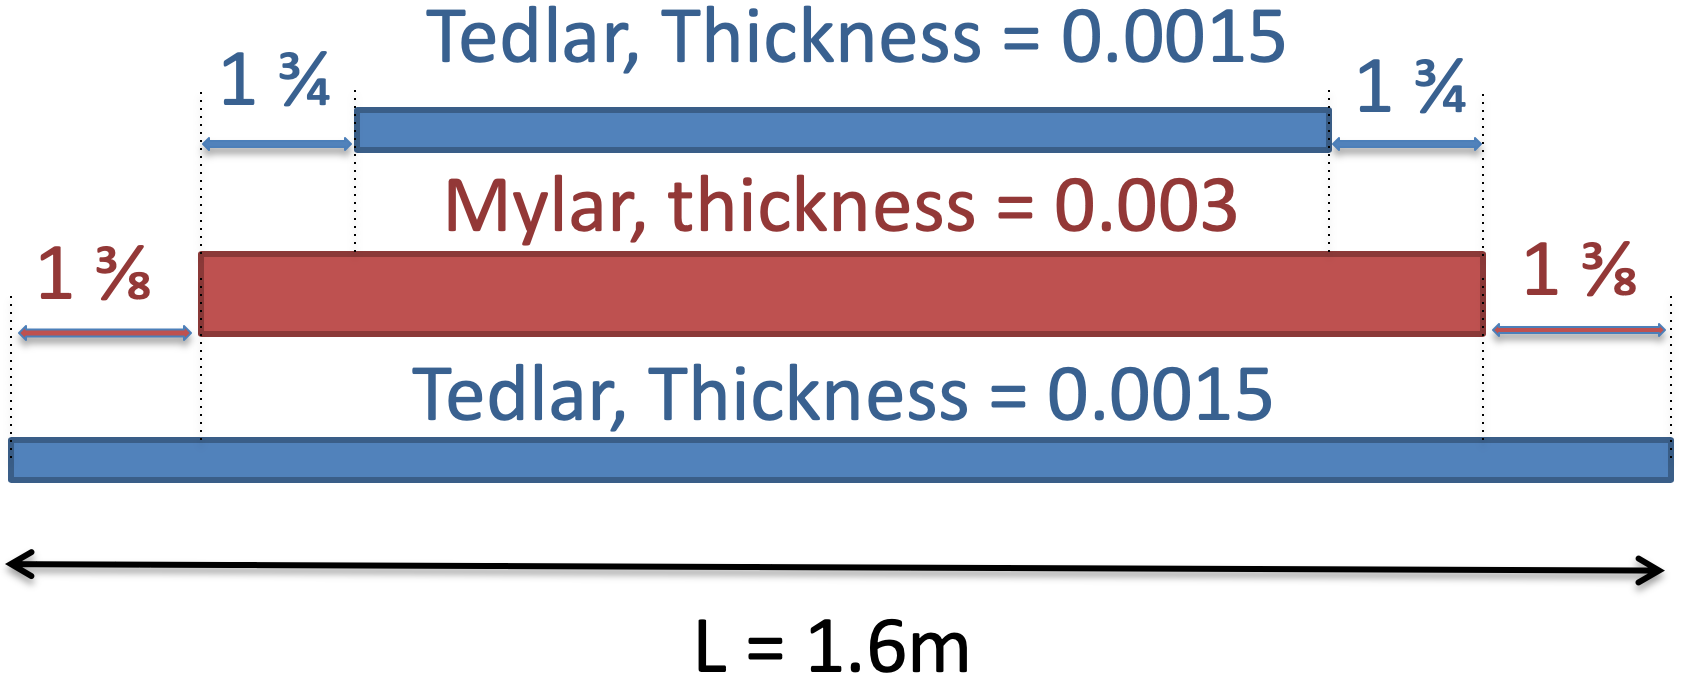
\includegraphics[width=1.0\columnwidth,keepaspectratio]{img/windowDesign.png}
	\caption{Top view of the back-wall of the LTCC. A stainless steel bar encapsulate a sandwich wall of aluminum and foam. On the left and right side
				 of the frame a new patch panel allow for 3 hermetical connectors (1 HV, 2 signals) from each PTM. }
	\label{fig:windowDesign}
\end{figure}



\paragraph{Lamination (company)}


\paragraph{Window tests}



\paragraph{Seaming (in house)}


\begin{figure}[h]
	\centering
	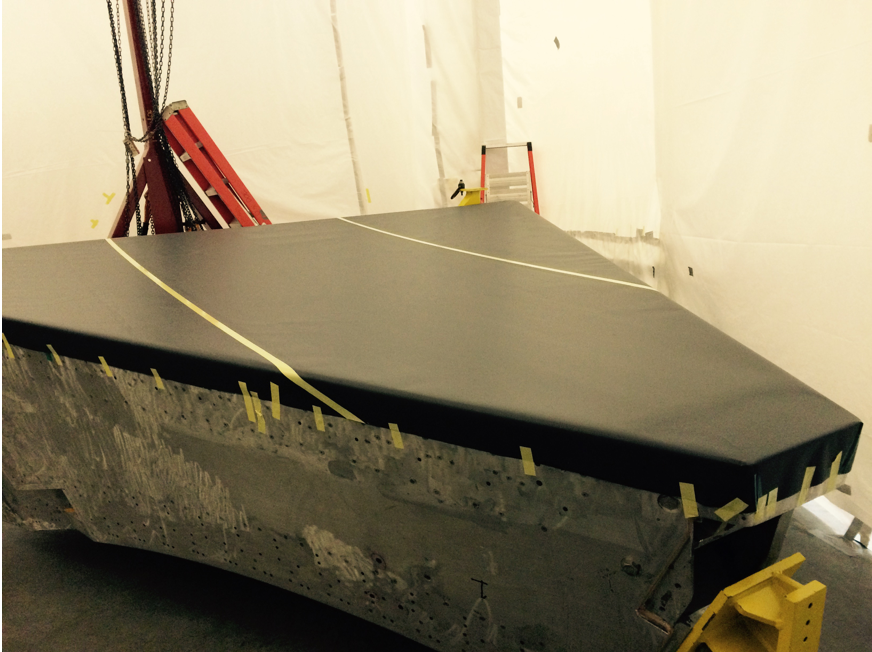
\includegraphics[width=1.0\columnwidth,keepaspectratio]{img/upstreamWindow.png}
	\caption{Top view of the back-wall of the LTCC. A stainless steel bar encapsulate a sandwich wall of aluminum and foam. On the left and right side
				 of the frame a new patch panel allow for 3 hermetical connectors (1 HV, 2 signals) from each PTM. }
	\label{fig:upstreamWindow.png}
\end{figure}




- Window to box glue + sealant

